\documentclass[11pt]{article}
\usepackage[margin=0.9in]{geometry}
\usepackage{amsmath,amssymb,amsthm,booktabs,array,hyperref,graphicx}
\hypersetup{colorlinks=true,linkcolor=blue,citecolor=blue,urlcolor=blue}
\setlength{\emergencystretch}{3em}
\newtheorem{theorem}{Theorem}
\newtheorem{lemma}{Lemma}
\newcommand{\diag}{\operatorname{diag}}
\newcommand{\Cov}{\operatorname{Cov}}
\newcommand{\Var}{\operatorname{Var}}
\title{Collective Mpemba cooling beyond triplet tests:\\a counterexample and a sharp amplitude bound}
\author{}
\date{12 October 2026}
\begin{document}
\maketitle
\begin{abstract}
Can tests on every three-state subsystem exclude anomalous cooling of a
four-state thermalizing system? We give a strictly positive reversible
generator that fails every original-rate triplet test in the proposed
finite-temperature protocol, yet exhibits ordinary Mpemba cooling between
two finite initial temperatures. Its rational slow eigenpair allows exact
verification of the triplet failures and the reversal in relaxation
distance. The mechanism is dilution of the slow-mode overlap by a
high-energy state whose mode component is nearly zero. A controlled rate
family turns this mechanism into a sharp onset criterion. Under the same
triplet-failure premise, we prove that the four-state slow-amplitude
advantage is strictly less than $25\%$ and construct admissible families
approaching this limit. The bound follows from a restriction on the first
three components of the slow eigenfunction and the Gibbs mass carried by
those states. Lean verifies the rational counterexample, its eventual
Pearson chi-square distance reversal, and the sharp amplitude supremum.
The result concerns slow amplitudes, not a universal fractional reduction
in cooling time.
\end{abstract}

\section{Introduction}
In Markovian relaxation, a preparation farther from equilibrium can lose
its long-lived component more effectively than a closer preparation. The
spectral account of the Mpemba effect makes this possibility precise:
initial temperature controls the overlap with the slow relaxation mode,
while the bath fixes the dynamics~\cite{lu,klich}. A practical question is
whether the absence of an effect in small subsystems can certify its
absence in a larger system.

Avitan, Factor and Gelbwaser-Klimovsky proposed an original-rate triplet
protocol for this purpose~\cite{avitan}. Its finite-temperature extension
infers absence in the full system when every energy-ordered triplet fails
a specified necessary-condition test. The inference is a conjecture in
that regime. The accompanying zero-temperature theorem uses stronger
hypotheses. A later protocol distinguishes exact three-state mechanisms
from the earlier necessary-condition predicate~\cite{protocol}; that
distinction matters when testing the original conjecture.

We resolve the four-state inference in its regular domain: distinct
energies, strictly positive reversible rates, a finite positive bath and
a simple slow mode. The inference fails even with strict triplet
inequalities and finite cooling preparations. We then explain why it
fails and quantify how much ordinary cooling can remain hidden from the
tests. The same premise that permits the counterexample enforces a sharp
$25\%$ upper bound on the slow-amplitude advantage.

The main text follows these three results: an exact witness, a predictive
mechanism and the sharp bound. Figure~\ref{fig:overview} connects them.
The companion \emph{Technical appendices} retain full algebraic proofs,
the second counterexample, broader classifications, higher-dimensional
extensions and the verification record. The original comprehensive
research report is preserved separately. The physical tools used here,
including reversible symmetrization, slow-mode projection and Perron
theory, are established; the contribution concerns their consequences
under this particular triplet premise.

\section{The model and the precise triplet premise}\label{sec:model}
Use column probability vectors, so $\dot p=Mp$ and $a_{ij}=M_{ij}$ is the
rate from $j$ to $i$ for $i\ne j$. The diagonal is
$M_{jj}=-\sum_{i\ne j}a_{ij}$. Let
\[
 E_1<E_2<E_3<E_4,\quad q_i=e^{-\beta_bE_i},\quad
 Q=\sum_iq_i,\quad \pi_b=q/Q,
\]
and impose detailed balance $M_{ij}q_j=M_{ji}q_i$. We assume every
off-diagonal rate is positive. Shifting the energy origin and measuring
energy in bath units set $E_1=0$ and $\beta_b=1$ without restricting the
energy spacings. A common rate multiplier changes only the time unit.

For an ordered triplet $i<j<k$, retain the full system's original rates
and define
\[
 A=a_{ik},\quad B=a_{jk},\quad C=a_{ij},\quad
 t=q_j/q_i,\quad u=q_k/q_j,
\]
\begin{align}
 \kappa&=\frac{A+B}{C(1+t)},\qquad G=At-B,\nonumber\\
 F&=A(1+tu/2)-B(1+u/2)-C(1-t).
\end{align}
The published necessary-condition predicate is
\begin{equation}\label{eq:predicate}
 P_{ijk}=(\kappa\geq1\ \land\ F>0)
       \ \lor\ (\kappa\leq1\ \land\ G>0).
\end{equation}
Both branch comparisons are inclusive, and both sign comparisons are
strict. No effective rates are substituted. If an isolated triplet
generator is formed, its diagonals must be recomputed to conserve
probability; a principal submatrix is not that generator.

\begin{lemma}[Exact branch reduction]\label{lem:cone}
For positive rates and ordered energies,
\[
 \neg P_{ijk}\quad\Longleftrightarrow\quad F_{ijk}\leq0,
 \quad G_{ijk}\leq0.
\]
\end{lemma}
\begin{proof}
Set $H=A+B-C(1+t)$, $d=(1-t)/(1+t)>0$ and
$h=2/(1+t)+u/2>0$. Direct expansion gives $F=hG+dH$.
If $H>0$, failure means $F\leq0$, which forces $G<0$.
If $H<0$, failure means $G\leq0$, which forces $F<0$.
At $H=0$, both branches apply and $F=hG$. These cases also prove the
converse and include $\kappa=1$.
\end{proof}
At fixed bath weights the premise is therefore eight closed linear
inequalities in the six downward rates, intersected with the positive
orthant. Equality faces belong to the original premise, although the
individual counterexample below lies strictly inside it.

Let $\lambda_2<0$ be the simple slowest nonzero eigenvalue and choose
$w^\top M=\lambda_2w^\top$, $Mv=\lambda_2v$, $w^\top v=1$.
Then $w^\top\pi_b=0$, and the slow overlap of a Gibbs preparation is
\begin{equation}\label{eq:overlap}
 b(\beta)=w^\top\pi(\beta),\qquad
 \pi_i(\beta)=\frac{e^{-\beta E_i}}{\sum_je^{-\beta E_j}}.
\end{equation}
For $0<\beta_h<\beta_c<1$, ordinary anomalous cooling means
$|b(\beta_h)|<|b(\beta_c)|$ with nonzero overlaps. Define its amplitude
advantage by
\begin{equation}\label{eq:advantage}
 \mathcal A=1-\frac{|b(\beta_h)|}{|b(\beta_c)|}.
\end{equation}
The conjectured implication would exclude every such pair whenever all
four predicates~\eqref{eq:predicate} fail. A single witness in this
restricted domain suffices to refute that general finite-temperature
inference. It does not challenge the zero-temperature theorem or the
three-state necessary condition itself.

\section{An exact four-state counterexample}\label{sec:witness}
\begin{theorem}[Strict triplet failure with ordinary cooling]\label{thm:witness}
There is a positive reversible four-state generator with distinct ordered
energies, a finite bath and a simple slow mode for which all four
original-rate triplet predicates fail strictly, yet the preparations
$\beta_h=1/1000$ and $\beta_c=1/100$ exhibit an initial-to-eventual
relaxation-distance reversal.
\end{theorem}
Take
\begin{equation}\label{eq:witnessdata}
 q=(1,199/200,2/5,1/400),\quad
 E=(0,\log(200/199),\log(5/2),\log400).
\end{equation}
The downward rates, in order $(12,13,14,23,24,34)$, are
\begin{equation}\label{eq:rates}
 \left(1,28,\frac{249}{10},
 \frac{330154675693}{1470375000},\frac{4983}{200},
 \frac{1527327066}{151990625}\right).
\end{equation}
Set $a_{ji}=a_{ij}q_j/q_i$ for $i<j$ and use conservative diagonals.
These formulas specify all entries of $M$ exactly. They immediately give
positive rates, detailed balance and column conservation; equilibrium is
$\pi_b=(400,398,160,1)/959$.

The following rational bounds summarize exact evaluation of the original
predicates. They are sign certificates, not rounded numerical tests.
\begin{center}
\begin{tabular}{cccc}
\toprule Triplet & Branch & Bound on $F$ & Bound on $G$\\\midrule
$123$ & $\kappa>1$ & $F<-230$ & $G<-196$\\
$124$ & $\kappa>1$ & $F<-1/50$ & $G<-13/100$\\
$134$ & $\kappa<1$ & $F<-19/10$ & $G<-2/25$\\
$234$ & $\kappa<1$ & $F<-118$ & $G<-3/100$\\\bottomrule
\end{tabular}
\end{center}
All four tests fail, with both branches represented. The exact
eigenfunction and eigenvalue are
\begin{equation}\label{eq:eigenpair}
 w=\left(1,-\frac{759}{1000},-\frac{48957}{80000},-\frac1{250}\right),
 \qquad \lambda_2=-\frac{4966671}{250000}.
\end{equation}
Rational multiplication verifies $M^\top w=\lambda_2w$ and $q^\top w=0$.
The paired right mode $v=\diag(q)w/N$ has $w^\top v=1$, where
\[
N=\sum_iq_iw_i^2=\frac{27567998009}{16000000000}.
\]

The characteristic polynomial factors into $x$, $250000x+4966671$, and
a quadratic with one root in each of $(-337,-336)$ and $(-60,-59)$.
Opposite exact endpoint signs locate both quadratic roots; they exhaust
its degree. Thus the displayed eigenvalue in $(-20,-19)$ is the simple
slow mode, separated from the other nonstationary modes by more than 39.
The quadratic and its rational coefficients are printed in the technical
appendix on the rational companion.

Integer-power enclosures for $q_i^{1/1000}$ and $q_i^{1/100}$ give
\begin{align}
 b(1/1000)&\in(-0.093755177882,-0.093755177881),\label{eq:intervals}\\
 b(1/100)&\in(-0.093857287853,-0.093857287852).\nonumber
\end{align}
Both overlaps are nonzero and negative, with the hotter preparation
having the smaller absolute value. Every displayed decimal endpoint is
a rational number whose enclosing inequalities are checked exactly.
Lean independently establishes wider, disjoint intervals sufficient for
the same conclusion. The amplitude advantage for this witness is about
$0.10879\%$; its role is to establish strict failure of the implication.

\subsection{From a slow overlap to an actual distance reversal}
For this generator define
\begin{equation}\label{eq:distance}
 D_q(p)=\sum_i\frac{(p_i-\pi_{bi})^2}{q_i}.
\end{equation}
It is a positive multiple of Pearson chi-square divergence and the square
of a weighted Euclidean norm. Reversible spectral evolution gives
\begin{equation}\label{eq:spectral}
 p(t;\beta)-\pi_b=e^{\lambda_2t}b(\beta)v+O(e^{\lambda_3t}),
 \qquad \lambda_3<\lambda_2.
\end{equation}
Consequently
\[
 \lim_{t\to\infty}\frac{D_q(p(t;\beta_h))}{D_q(p(t;\beta_c))}
 =\frac{b(\beta_h)^2}{b(\beta_c)^2}<1.
\]
For the two specified preparations, exact bounds also give
$D_q(\pi(1/100))<24<D_q(\pi(1/1000))$.
The hotter preparation therefore starts farther away and becomes closer
for every sufficiently large time. Continuity ensures a crossing at a
finite positive time. Lean proves the evolution's master equation and
uniqueness, its spectral limit and these two distance orderings; the
argument does not assume a numerical eigenvector or crossing time.

The conventional KL conclusion follows analytically from
\[
 D_{\rm KL}(p(t;\beta)\Vert\pi_b)
 =\frac12e^{2\lambda_2t}b(\beta)^2
       \sum_i\frac{v_i^2}{\pi_{bi}}+o(e^{2\lambda_2t}),
\]
and $\partial_\beta D_{\rm KL}(\pi(\beta)\Vert\pi_b)
=(\beta-1)\Var_{\pi(\beta)}(E)<0$ on cooling.
This KL bridge is not part of the Lean verification. Nor does the overlap
comparison identify the earliest crossing or imply a reversal at every
time. Figure~\ref{fig:overview}A illustrates the quadratic-distance
evolution numerically.

\begin{figure}[t]
\centering
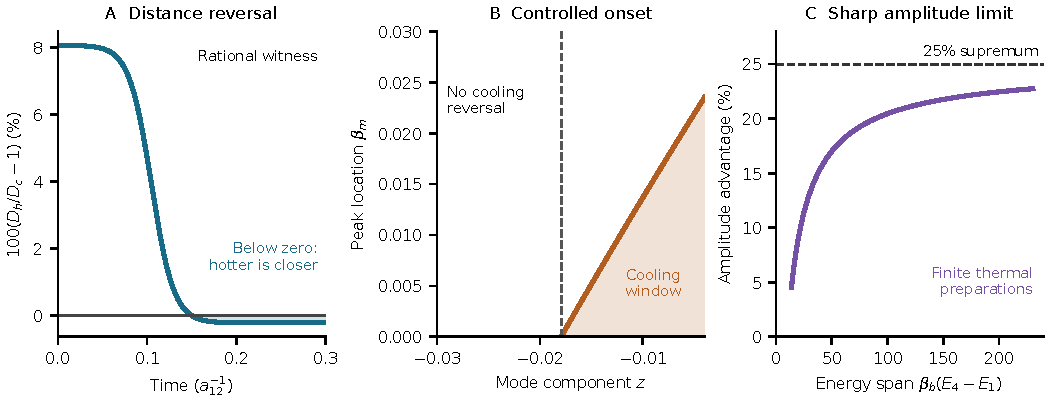
\includegraphics[width=\textwidth]{output/figures/focused_overview.pdf}
\caption{\textbf{Counterexample, mechanism and bound.}
\textbf{A:} Actual $D_q$ relaxation for the rational generator in
Eqs.~\eqref{eq:witnessdata}--\eqref{eq:rates}, with
$\beta_h=1/1000$ and $\beta_c=1/100$. The sign changes from hotter-farther
to hotter-closer; the late-time ratio difference approaches $-0.21747\%$.
\textbf{B:} Varying the highest-state mode component $z$ in the controlled
family produces an anomalous interval $0<\beta<\beta_m(z)$ only above
$z_*\simeq-0.0179401112$. Every triplet still fails throughout this family.
\textbf{C:} A different family approaches the sharp $25\%$ amplitude
supremum as its energy span grows. Here
$\beta_h=[\log(1/\varepsilon)]^{-2}$ and $\beta_c$ is the numerical
overlap maximum. Curves are high-precision illustrations of separately
proved claims. Panel A does not certify a numerical crossing bracket;
panel C concerns amplitude, not cooling-time reduction.}
\label{fig:overview}
\end{figure}

\section{The mechanism: a nearly neutral high-energy state}\label{sec:mechanism}
The slow eigenfunction in Eq.~\eqref{eq:eigenpair} assigns a positive
value to the ground state, appreciably negative values to the two middle
states and an almost zero value to the highest state. At high initial
temperature, population in the highest state dilutes the negative mean
overlap. A slightly cooler preparation depopulates that state and
increases the magnitude of the mean. Further cooling transfers weight
to the ground state and brings the overlap back to zero at the bath.
This is a collective projection effect: each isolated triplet has its own
eigenfunction and normalization, so its test cannot constrain the full
four-state Gibbs projection in the required way.

This explanation can be made predictive by designing a rate family with
the desired mode. Keep Eq.~\eqref{eq:witnessdata} and four of the rates,
and set
\begin{align}
 w(z)&=(1,-p,-r_0-\eta z,z),\label{eq:family}\\
 p&=759/1000,\qquad r_0=48959/80000,\qquad \eta=1/160,\nonumber\\
 -3/100&\leq z\leq-1/250.\nonumber
\end{align}
The small adjustment in the third component enforces $q^\top w(z)=0$.
Choose
\begin{align}
 a_{23}(z)&=\frac{528238451563-2257386450z}
                    {200000(11761-500z)},\label{eq:familyrates}\\
 a_{34}(z)&=\frac{2(1550z^2-5989657z+1197903)}
                    {5(80500z+48959)},\nonumber
\end{align}
while $a_{12}=1$, $a_{13}=28$, $a_{14}=249/10$ and
$a_{24}=4983/200$. Upward rates and diagonals follow as before.
Then $M(z)^\top w(z)=\lambda(z)w(z)$ exactly, where
$\lambda(z)=-(1550z+3973343)/200000$.
At $z=-1/250$ this is the counterexample in Section~\ref{sec:witness}.

Throughout the closed parameter interval all rates are positive, all
four triplets fail strictly, and $w(z)$ is the simple slow mode. These
are interval-wide statements: rational Bernstein sign certificates verify
the rate and triplet inequalities. A reversible comparison with the
baseline rates $a_{23}=224$, $a_{34}=10$ places two eigenvalues below
$-50$, whereas $-20<\lambda(z)<-19$. Thus the prescribed vector is not
accidentally a fast mode. Full certificates are in the mechanism appendix.

\subsection{An exact onset criterion}
Write $r=r_0+\eta z$ and $E_\Sigma=E_2+E_3+E_4$. In this family
$p>r>-z>0$, $E_4>E_2+E_3$, and
$(1+r)E_3>(p-r)(E_3-E_2)$. The numerator
$N(\beta)=\sum_iw_i e^{-\beta E_i}$ has $N'(\beta)>0$ and
$N(1)=0$, hence $b(\beta)<0$ on cooling. Put
\[
 D(\beta)=Z(\beta)^2b'(\beta),\qquad
 J(\beta)=e^{\beta E_4}D(\beta).
\]
Define $c_{1j}=(w_1-w_j)E_j>0$ and
$c_{ij}=(w_j-w_i)(E_j-E_i)>0$ for $2\leq i<j\leq4$.
The pair expansion of the covariance gives
\begin{align}
 J(\beta)={}&c_{12}e^{\beta(E_4-E_2)}
 +e^{\beta(E_4-E_2-E_3)}(c_{13}e^{\beta E_2}-c_{23})\nonumber\\
 &+c_{14}-c_{24}e^{-\beta E_2}-c_{34}e^{-\beta E_3}.\label{eq:monotoneJ}
\end{align}
Because $c_{13}>c_{23}$, every nonconstant term is strictly increasing
for $\beta\geq0$, and $J(1)>0$. Thus an absolute-overlap maximum occurs
on $0<\beta<1$ exactly when $J(0)<0$, and it is unique.
This monotonicity argument is needed: an endpoint derivative alone would
not generally exclude another turning point.

Set
\begin{align}
 U&=(1-p-r_0)E_\Sigma+4(pE_2+r_0E_3),\nonumber\\
 V&=(3+\eta)E_4-(1-\eta)E_2-(1+3\eta)E_3>0.
\end{align}
Direct evaluation yields $J(0)=U-Vz$. Hence
\begin{equation}\label{eq:onset}
 \text{ordinary asymptotic cooling exists}\quad\Longleftrightarrow\quad
 z>z_*:=U/V,
\end{equation}
with the certified bracket $-0.017940112<z_*<-0.017940111$.
For $z\leq z_*$, $|b|$ decreases throughout cooling. For $z>z_*$,
the interval $0<\beta<\beta_m(z)$ has increasing $|b|$ and supplies
finite-temperature witnesses. Infinite temperature is used only as an
analytic endpoint, not as an initial preparation.

The fixed pair $(1/1000,1/100)$ reverses only for
$z>z_{\rm pair}\simeq-0.01480024798314$. Between $z_*$ and
$z_{\rm pair}$ the effect exists but this pair misses it. Near onset,
with $d_*=\partial_\beta D(0,z_*)>0$ and $\delta=z-z_*$,
\[
 \beta_m=\frac{V}{d_*}\delta+O(\delta^2),\qquad
 |b(\beta_m)|-|b(0)|=\frac{V^2}{32d_*}\delta^2+O(\delta^3).
\]
The anomalous temperature window opens linearly, while its amplitude
advantage is initially quadratic. This explains why a finite temperature
grid can miss the onset without implying absence.

\section{Why every such four-state advantage is below 25\%}\label{sec:bound}
The mechanism suggests a four-to-three-state normalization effect.
The following theorem proves that the triplet premise permits no larger
ordinary cooling amplitude advantage, regardless of energy spacings or
rate ratios.

\begin{theorem}[Sharp amplitude bound]\label{thm:bound}
Let a positive reversible four-state generator have distinct ordered
energies, a finite positive bath and a simple slow mode. If all four
original predicates~\eqref{eq:predicate} fail, then for every
$0<\beta_h<\beta_c<\beta_b$,
\begin{equation}\label{eq:bound}
 \frac{|b(\beta_c)|}{|b(\beta_h)|}<\frac43,
 \qquad \mathcal A<\frac14.
\end{equation}
The value $1/4$ is the supremum of attainable ordinary cooling advantages
under these hypotheses and is not attained at finite admissible parameters.
\end{theorem}

The proof separates a restriction on the eigenfunction from a thermal
normalization inequality. The eigenfunction restriction is the step at
which the full $F,G$ premise is essential.

\begin{lemma}[First-three mode restriction]\label{lem:shape}
Under Theorem~\ref{thm:bound}'s hypotheses, the slow mode can be oriented
so that its overlap is negative on $0<\beta<\beta_b$ and
\begin{equation}\label{eq:shape}
 w_1\geq w_2,\qquad w_1+w_2\geq2w_3,\qquad w_4\leq0.
\end{equation}
\end{lemma}
To describe the structural argument, let $Q_k=\sum_{i\leq k}q_i$ and
use the three bath-orthogonal prefix contrasts
\[
 h^{(k)}_i=\begin{cases}
 1,&i\leq k,\\-Q_k/q_{k+1},&i=k+1,\\0,&i>k+1.
 \end{cases}
\]
The conditions $G_{ijk}\leq0$ imply that the representation of $M^\top$
in the normalized contrast basis is symmetric with nonnegative
off-diagonal entries. Its largest eigenvector can be chosen nonnegative.
Each contrast has strictly negative Gibbs mean on cooling, so a nonzero
nonnegative combination has negative overlap. This also gives
$w_1\geq w_2$ and $w_4\leq0$.

The remaining inequality, $w_1+w_2\geq2w_3$, uses the $F$ constraints.
Subtract the smallest reversible reset component, which leaves $F,G$
unchanged and shifts all nonstationary eigenvalues equally. The residual
generator has nonnegative rates and at least one of its first-row
downward rates zero. Eliminate the third contrast coordinate by a
reversible Schur complement. The desired eigenvector ratio then reduces
to a polynomial nonnegativity statement on three exhaustive zero-rate
faces, each implied by the original inequalities. Simplicity supplies the
strict diagonal gap needed for elimination, including reducible residual
generators. The complete face calculation is in the sharp-bound appendix
and is formalized in Lean; no sign or mode-shape assumption is added to
the theorem's premise.

\begin{proof}[Thermal part of Theorem~\ref{thm:bound}]
Normalize $\beta_b=1$. Let $m(\beta)$ be the conditional Gibbs mean of
$w$ on states $1,2,3$. Equation~\eqref{eq:shape} expresses those three
mode values as a constant vector plus
\[
 u(1,-1,0)+v(1,1,-2),\quad
 u=(w_1-w_2)/2\geq0,\quad
 v=(w_1+w_2-2w_3)/6\geq0.
\]
Both nonconstant vectors have increasing conditional Gibbs mean with
inverse temperature. Explicitly, write $a=E_2$, $b=E_3$,
$t=e^{-\beta a}$, $y=e^{-\beta b}$ and
$(p_1,p_2,p_3)=(1,t,y)/(1+t+y)$. Then
\[
 (p_1-p_2)'=\frac{2at+by-(b-a)ty}{(1+t+y)^2}>0,
 \qquad (p_1+p_2-2p_3)'=-3p_3'>0.
\]
Here $0<t\leq1$ and $0<a<b$. Thus $m$ is nondecreasing.

Let $P(\beta)=Z_3(\beta)/Z_4(\beta)$ denote the mass on the first
three states. It increases strictly with $\beta$ and obeys
$3/4<P(\beta)<1$ at finite positive temperature. For
$r=P(\beta_c)/P(\beta_h)$, therefore $1<r<4/3$.
Since $b=Pm+(1-P)w_4$,
\[
 b(\beta_c)-r b(\beta_h)
 =P(\beta_c)[m(\beta_c)-m(\beta_h)]+(1-r)w_4\geq0.
\]
Both overlaps are negative, giving
$|b(\beta_c)|\leq r|b(\beta_h)|<(4/3)|b(\beta_h)|$.
This proves the strict bound. The construction below proves sharpness.
\end{proof}

The calculation identifies the physical bottleneck. Depopulating the
highest state can amplify the negative overlap of the first three, but
their conditional mean cannot become more negative as cooling proceeds.
Their probability mass can increase by a factor less than $4/3$ because
it already exceeds $3/4$ at every finite positive initial temperature.
That thermal restriction turns the local-rate constraints into a global
amplitude bound.

\section{Approaching the bound with admissible generators}\label{sec:sharpness}
Set
\begin{align}
 q_\varepsilon&=(1,1-\varepsilon/3,3/5,\varepsilon^2),\nonumber\\
 w_\varepsilon&=(1,-4/5,-1/3-4\varepsilon/9+5\varepsilon^3/3,-\varepsilon).
 \label{eq:sharpfamily}
\end{align}
The compensation in the third component makes $q_\varepsilon^\top
w_\varepsilon=0$. There are positive reversible generators with this
mode and $\lambda_2=-3$ for every sufficiently small positive
$\varepsilon$, and every original triplet predicate fails.
One construction fixes $a_{12}=1$ and defines the other rates by rational
functions. Their limits, in the order used in Eq.~\eqref{eq:rates}, are
\[
 (1,3/2,20/17,15/7,20/17,12/17).
\]
In this family $F_{124}=G_{234}=0$ identically. All rates and the
remaining required strict signs are controlled by continuity of explicit
rational functions at zero; the sign of the vanishing $G_{124}$ factor
is checked after extracting its positive factor $\varepsilon$.
A positive contrast eigenvector and two connecting positive entries
establish slow-mode simplicity. The exact rates and sign checks are in
the formal sharpness appendix and \path{formal/Mpemba/SharpFamily.lean}.
The singular bath at $\varepsilon=0$ is used only to compute limits;
every actual member uses $\varepsilon>0$.

To exhibit finite preparations approaching the bound, take a real
parameter $L\to\infty$ and set
\[
 \varepsilon=e^{-L^2},\qquad \beta_h=L^{-3},\qquad\beta_c=L^{-1}.
\]
For sufficiently large finite $L$, $0<\beta_h<\beta_c<1$.
The highest energy is $E_4=2L^2$. Consequently its unnormalized Gibbs
weight is $e^{-2/L}\to1$ in the hot preparation and
$e^{-2L}\to0$ in the cooler preparation, while the first three weights
tend to one in both. Meanwhile
$w_\varepsilon\to(1,-4/5,-1/3,0)$, and therefore
\[
 b_h\longrightarrow\frac{1-4/5-1/3}{4}=-\frac1{30},\qquad
 b_c\longrightarrow\frac{1-4/5-1/3}{3}=-\frac2{45}.
\]
Thus $\mathcal A\to1-(3/4)=1/4$. Lean proves that these are limits
of actual admissible family members, not merely of a conditional overlap
formula, and proves the least-upper-bound and nonattainment statements.

Equality in two triplet constraints is permitted by the original strict
predicate tests. A separate construction in the technical appendices
has the same limiting weights and eigenfunction, a slow eigenvalue fixed
at $-3$, and a gap exceeding $1/3$. A perturbation makes all eight
triplet inequalities strict while preserving a gap greater than $1/4$
and the same amplitude limit. Those stronger claims have analytic and
exact rational certificates but are outside the present Lean coverage.
Figure~\ref{fig:overview}C uses that unperturbed, uniformly gapped family;
the thermal geometry is common to both constructions.

The large advantage is accompanied by large energy separation. For
example, the separately certified finite choice $\varepsilon=10^{-50}$,
$\beta_h=1/10000$ and $\beta_c=1/50$ gives an amplitude advantage
between $22.6171597478\%$ and $22.6171597506\%$ before the strict
perturbation, and greater than $22\%$ afterwards. This is a finite
mathematical witness, not a demonstrated laboratory operating regime.

\section{Verification, interpretation and scope}\label{sec:verification}
The exact rates, eigenpair and triplet signs of Section~\ref{sec:witness}
can be checked using rational arithmetic. Integer-power inequalities
certify the thermal enclosures. The companion Lean library goes further:
it checks a complete quadratic-distance reversal under the master
equation and proves the sharp amplitude theorem for the full generator
under explicit spectral assumptions. In the general theorem,
\texttt{SimpleSlowMode} specifies a nonzero bath-orthogonal left
eigenfunction, its eigen-equation, a one-dimensional eigenspace and the
largest Rayleigh quotient on the bath-orthogonal subspace.

The main formal entry points are
\path{Mpemba.appendixB_counterexample},
\path{Mpemba.master_equation_distance_reversal}, and
\path{Mpemba.Quarter.sharp_quarter_isLUB}. The name ``Appendix B''
refers to the witness's location in the preserved research report; it is
the main counterexample of this focused paper. Lean checks the original
inclusive branch conditions, exact real Gibbs overlaps, slow-mode
simplicity, the evolution and its uniqueness, and the limiting family's
admissibility. It does not formalize the controlled onset theorem,
the general KL bridge, numerical crossing times, or the uniformly gapped
strict-triplet perturbation.

The library pins Lean 4.19.0 and mathlib commit
\path{c44e0c8ee63ca166450922a373c7409c5d26b00b}. With elan, Git,
Python 3 and a POSIX shell installed, preserve the committed dependency
manifest and run from the source-package root:
\begin{verbatim}
cd formal
lake exe cache get
./check.sh
\end{verbatim}
The first setup requires network access. Do not run \texttt{lake update}
to reproduce the pinned dependency set. The README supplies a Lean
interpreter fallback if the compiled cache downloader fails to link.
The verified build includes 27 proof modules and 43 named-theorem axiom
audits, with no admitted proofs or custom axioms. Successful execution
ends with
\begin{verbatim}
PASS: 43 theorem axiom audits; standard logical axioms only.
\end{verbatim}
The only permitted axiom dependencies are \texttt{propext},
\texttt{Classical.choice} and \texttt{Quot.sound}. Formal checking does
not establish priority or replace review of the correspondence between
the source conjecture and its transcription.

The asymptotic distance and time interpretations must be kept separate
from amplitude. For a quadratic distance, including the leading KL
term, $\mathcal A<1/4$ implies a limiting distance advantage below
$1-(3/4)^2=7/16$. For a vanishing common distance threshold, the
asymptotic time advance is
\[
 \Delta t=\frac{\log(|b_c|/|b_h|)}{|\lambda_2|}
 <\frac{\log(4/3)}{|\lambda_2|}.
\]
Both preparations retain the same slow exponent. This is an ordinary
effect and does not assert a $25\%$ reduction in total cooling time,
which depends on the chosen threshold and earlier dynamics.

The witness also does not contradict finite sampling within a restricted
parameter box: its bath-scaled energy span is $\log400>5$. Strict rates,
strict triplet signs, spectral separation and strict overlap reversal
give an open neighborhood of counterexamples by continuity. No numerical
radius for that neighborhood or experimental robustness claim is made.

\section{Discussion}
The failed inference is local-to-global: all original-rate triplet tests
can fail while the full system's slow eigenfunction still has anomalous
thermal ordering. The nearly neutral high-energy state explains this
possibility and supplies a rate-controlled onset. The full triplet
premise nonetheless constrains the slow eigenfunction strongly enough
to bound the four-state amplitude advantage sharply.

The distinction between the counterexample and the bound is useful.
The former disproves a universal absence claim with an interior witness;
the latter describes the entire regular four-state domain under that
premise. The limiting factor $4/3$ has a direct Gibbs-normalization
interpretation, and the matching construction shows that it cannot be
improved without additional assumptions.

The technical appendices retain the broader results: surviving
strong-effect and heating exclusions, finite-temperature classifiers,
degenerate-mode results, finite-time distance tests, inverse realization,
finite-span refinements and higher-dimensional constructions. These are
not needed to state the central four-state conclusion. A useful further
physical question is how much finite-time advantage remains when energy
spans and rates are constrained by a concrete thermalization model.

\paragraph{Availability.}
The accompanying source package contains this manuscript, the technical
appendices, the preserved comprehensive research report, exact Python
certificates, the Lean library and the overview figure's source and data.
\path{RUNME.txt} gives the document and verification build commands.
The figure is generated by \path{research/focused_overview.py}; its
curves are numerical illustrations, with exact claims supported by the
separate proofs and certificates described above.

\begin{thebibliography}{9}
\bibitem{lu} Z. Lu and O. Raz, Nonequilibrium thermodynamics of the
Markovian Mpemba effect and its inverse, \emph{Proc. Natl. Acad. Sci. USA}
\textbf{114}, 5083--5088 (2017),
\href{https://pmc.ncbi.nlm.nih.gov/articles/PMC5441807/}{full text}.
\bibitem{klich} I. Klich, O. Raz, O. Hirschberg and M. Vucelja,
Mpemba index and anomalous relaxation, \emph{Phys. Rev. X}
\textbf{9}, 021060 (2019),
\href{https://doi.org/10.1103/PhysRevX.9.021060}{doi:10.1103/PhysRevX.9.021060}.
\bibitem{avitan} I. Avitan, R. Factor and D. Gelbwaser-Klimovsky,
Necessary conditions for the Markovian Mpemba effect,
\href{https://arxiv.org/abs/2603.04567v1}{arXiv:2603.04567v1} (2026),
Eq.~(3), the $N$-level protocol and supporting information S2--S14.
\bibitem{protocol} D. Gelbwaser-Klimovsky,
Efficient protocol for the Markovian Mpemba effect in $N$-level systems,
\href{https://arxiv.org/abs/2609.09988v1}{arXiv:2609.09988v1} (2026),
Sec.~II.
\end{thebibliography}
\end{document}
